\newpage
\subsection{Volume Rendering}

Unter dem Begriff Volume Rendering befindet sich eine Reihe von Methoden, die es ermöglichen ein 3D-Datenset zu visualisieren.
Anders als beim Rendern von Geometrien mit einer festen Oberfläche, geht es hierbei darum alle Daten aus
dem jeweiligen Volumen darstellen zu können. Dies sind beispielsweise volumetrische Effekte wie Feuer und Rauch, Wolken oder Nebel,
welche sich, aufgrund ihrer gasförmigen Eigenschaften, nicht wirklich realistisch mit Geometrie darstellen lassen.
Eine Rauchwolke hat keine wirkliche Oberfläche, sondern besteht aus unzähligen winzigen Rußpartikeln.
Möchte man also solche Volumen darstellen, so geraten die bisherigen Herangehensweisen, die sich die Oberflächen der Objekte zunutze machen,
schnell an ihre Grenzen. Beim Grundgedanken des Volume Renderings geht es daher um die Frage, wie das Licht durch diese Volumen
wandert und welchen Einfluss die Partikel darauf haben.
Es gibt einige Faktoren, die beeinflussen was das Auge am Ende von diesem Volumen sieht. Wenn das Licht durch solch ein Volumen wandert
kann es absorbiert, reflektiert oder gestreut werden.
Die Abschwächung durch Streuung und Absorption des Lichtes beim Durchlaufen eines Volumens kann mithilfe des Lambert-beerschen Gesetzes wie in \ref{eqn:beer} 
approximiert werden \parencite{Mayerhofer2020}. 
Der Absorptionskoeffizient $\sigma_a$ beschreibt dabei die Wahrscheinlichkeit, dass ein Photon auf der Strecke $d$ durch das Medium absorbiert wird. 

\vspace{-0.5cm  }
\begin{equation} 
    \label{eqn:beer}
    I_{out} = I_{in} \cdot e^{- ( d \cdot\sigma_a  )}.
\end{equation}




\subsubsection{Ray Marching}

Ray Marching ist eine dieser Möglichkeiten ein Volumen darzustellen. Die Idee hierbei ist es – ähnlich wie beim Ray Tracing – 
Strahlen von der Kamera aus durch jeden Pixel des zu rendernden Bildes zu schicken und dabei zu prüfen, ob der Strahl auf etwas trifft.
Der Unterschied besteht hierbei jedoch darin, dass sich Ray Marching auf sogenannten '\textit{signed distance functions}' (SDF) beruht.
SDFs beschreiben, wie weit die nächstgelegene Oberfläche entfernt ist. Befindet sich der Strahl noch außerhalb der Geometrie, so ist 
der Wert der Funktion positiv, befindet sich der Strahl innerhalb, so wird der Wert negativ. Dazu wird die Entfernung zu allen Objekten 
in der Szene berechnet.

\begin{figure}[h]
	\centering
	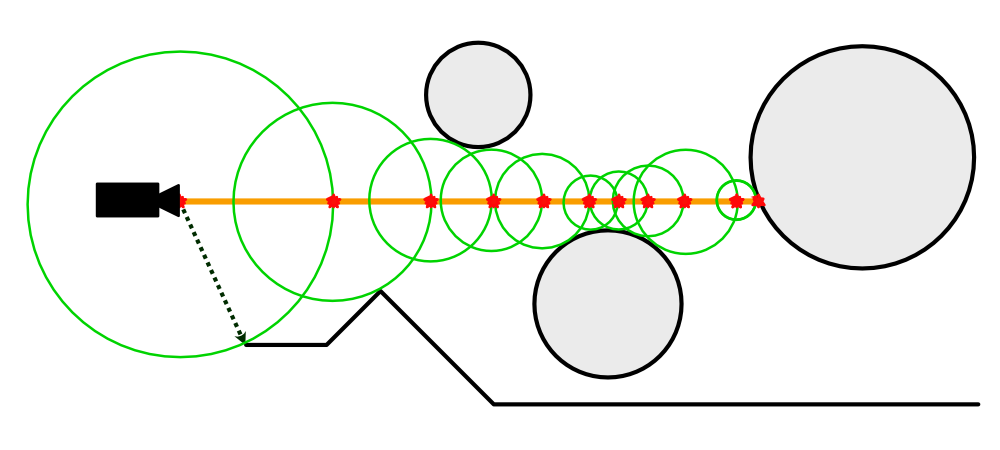
\includegraphics[width=0.80\textwidth]{Grafiken/Basics/Volume/Sphere_Tracing.png}
	\begin{footnotesize}
		\caption{Sphere Tracing: Der Algorithmus wird so lange wiederholt, bis der Radius/Abstand zum nächstgelegenen
        Objekt unter einen bestimmten Grenzwert fällt.}
	\end{footnotesize}
\end{figure}



Im ersten Schritt muss also die Distanz zur nächstgelegenen Oberfläche gefunden werden. Daraus ergibt sich ein Radius in dem sich 
mit Sicherheit nichts anderes befindet. Der Strahl bewegt sich nun um die Länge des berechneten Radius' in seine vorgesehene Richtung.
Nun werden diese beiden ersten Schritte an der neuen Position wiederholt. Dies passiert so lange, bis die Entfernung gegen einen festgelegten
Grenzwert geht. Dies deutet darauf hin, dass eine Oberfläche getroffen wurde. Diese Variante von Ray Marching wird auch 
'\textit{Sphere Tracing}' genannt. Sphere Tracing ist, im Gegensatz zu einer konstanten Schrittweite, ein effizienter Algorithmus um 
Oberflächen entlang des Strahls zu finden, da hiermit die Anzahl der benötigten Schritte deutlich reduziert werden kann. 


\subsubsection{Volume Ray Marching}

\begin{figure}[h]
	\centering
    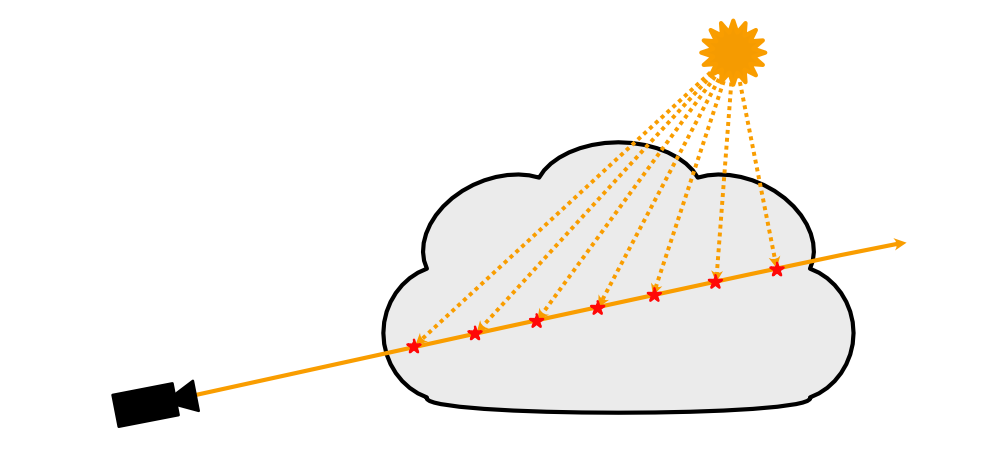
\includegraphics[width=0.80\textwidth]{Grafiken/Basics/Volume/Volume_RayMarching.png}
	\begin{footnotesize}
		\caption{Vereinfachte Darstellung des Volume Ray Marching. Der Weg des Lichtes durch 
        das Medium in der Realität aufgrund von In-/ und Out-Scattering oder Emissionen innerhalb des
        Volumens komplexer.}
	\end{footnotesize}
\end{figure}


Wurde eine Oberfläche gefunden, so wird in festgelegten Schritten (sample rate) das Volumen durchlaufen und an jedem Schritt das Licht berechnet.



% \subsubsection{Texturbasierte Volumen}